\documentclass[12pt]{amsart}
\usepackage{amsfonts, amssymb, latexsym, epsfig, graphicx}

\setlength{\oddsidemargin}{0in}
\setlength{\evensidemargin}{0in}
\setlength{\marginparwidth}{0in}
\setlength{\marginparsep}{0in}
\setlength{\marginparpush}{0in}
\setlength{\topmargin}{0in}
\setlength{\headheight}{0in}
\setlength{\headsep}{.3in}
\setlength{\footskip}{.3in}
\setlength{\textheight}{9in}
\setlength{\textwidth}{6.5in}
\setlength{\parskip}{4pt}

\newcommand{\Q}{\mathbb{Q}}
\newcommand{\N}{\mathbb{N}}
\newcommand{\R}{\mathbb{R}}
\newcommand{\Z}{\mathbb{Z}}

\begin{document}

{\large Spencer Butler}

{\large Real-time Operating Systems}

{\large Stepper Motor Project}



\section{Program Description}

\subsection{Overview}

The program controls both a spinning dial and a display to indicate values. The dial and the display
have independent states controlling what they indicate. These states are reached by pressing buttons,
according to the Operator Instructions.

\newpage
\subsection{Diagrams}

$$ $$

\begin{figure}[h!]
    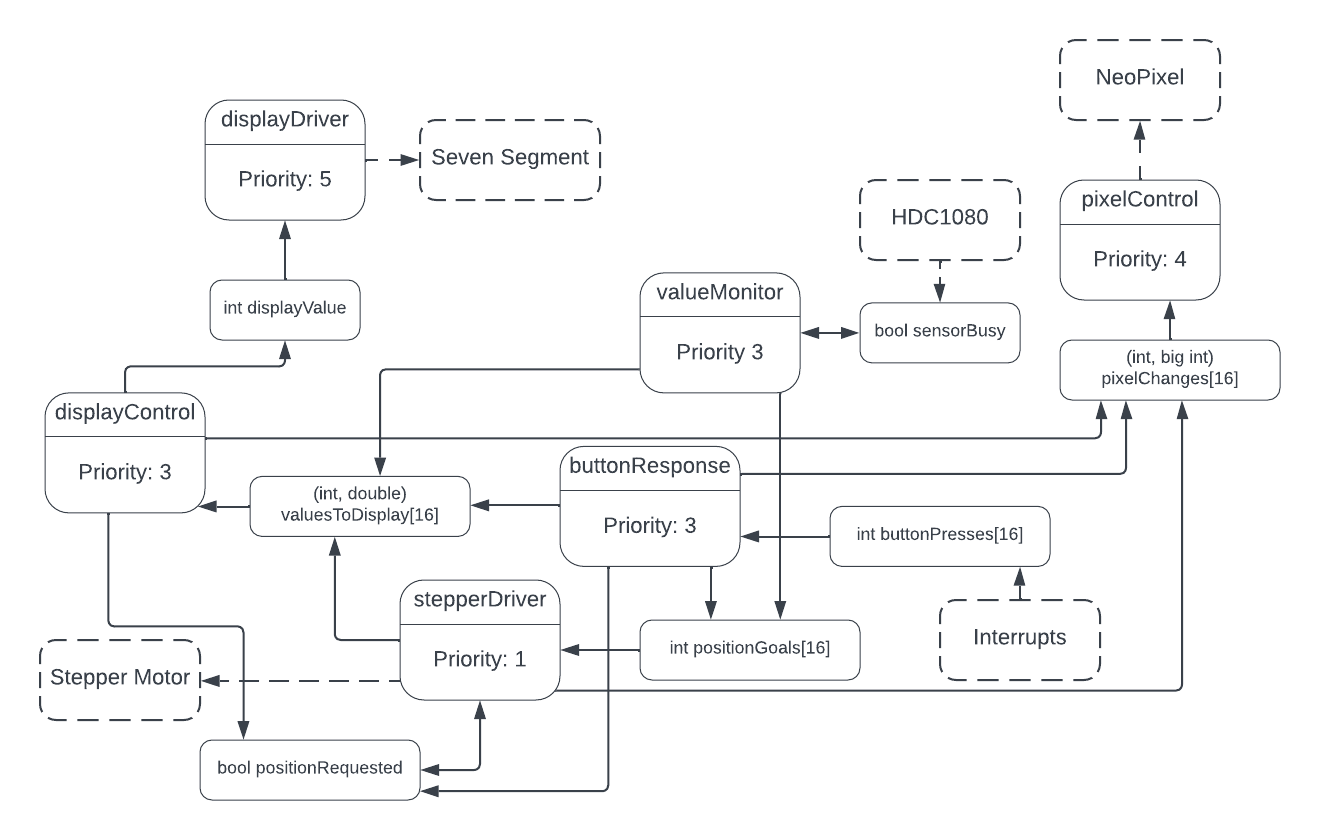
\includegraphics[width=7in]{stepperBlockDiagram}
    \caption{Block diagram showing tasks with priority and main interactions/dataflow.}
\end{figure}


\subsection{Operator Instructions}

\subsubsection{Dial Controls}

The dial can be set to track different variables, or to move a specific way, via pressing
specific buttons a certain number of consecutive times. Changes will take immediate effect.

\begin{center}
    \begin{tabular}{c|c|c}
        Button & Number of Presses & Effect on Dial \\
        \hline
        1 & 1 & Dial tracks measured humidity \\
        1 & 2 & Dial tracks measured temperature \\
        2 & 1 & Dial rotates clockwise continually \\
        2 & 2 & Dial rotates counterclockwise continually \\
        2 & 3 & Dial alternately rotates clockwise and counterclockwise \\
    \end{tabular}
\end{center}


\subsubsection{Display Controls}

The display can be set to show different variables via pressing buttons. Each value on the
display persists for several seconds, so changes are queued to take effect after other
values have been displayed. If too many values are queued at once, the display will show 0F for
Overflow.

\begin{center}
    \begin{tabular}{c|c|c}
        Button & Number of Presses & Effect on Display \\
        \hline
        3 & 1 & Display shows measured temperature \\
        3 & 2 & Display shows measured humidity \\
        3 & 3 & Display shows position of dial \\
        1 & 4 & Toggle display between hex and decimal \\
    \end{tabular}
\end{center}

\subsubsection{Special Controls}

Making 3 consecutive presses of button 1 will clear the display and the dial.
While the display is thus cleared, it will display EE. The display and dial will
each require inputting a new directive to resume showing some variable.

Flipping the leftmost switch will cause the LEDs to perform a rainbow animation, rather than
showing information as normal.

\subsubsection{Indicator LED Interpretation}

Each of the four LEDs displays a specific program state, unless they are currently performing the
rainbow animation.

\begin{center}
    \begin{tabular}{c c}
        \hline
        LED 1 (Top) & \\
        Yellow & Display shows temperature \\
        Blue & Display shows humidity \\
        Green & Display shows dial rotation \\
        White & Display is not showing a value \\
        \hline
        LED 2 & \\
        Yellow & Display is in hexadecimal \\
        Blue & Display is in decimal \\
        White & Display is not showing a value \\
        \hline
        LED 3 & \\ 
        Yellow & Dial tracks temperature \\
        Blue & Dial tracks humidity \\
        Green & Dial alternates clockwise and counterclockwise rotations \\
        White & Dial does not indicate a value \\
        \hline
        LED 4 & \\
        Green & Dial position is stable \\
        Red & Dial position is unstable \\
    \end{tabular}
\end{center}

\section{Task Descriptions}

\subsection{Value Monitor}

This task periodically retrieves temperature and humidity data from the HDC1080 sensor.
If either the motorGoal or displayType state variables are set to either temperature or
humidity, it then sends the data to the appropriate queues. Additionally, it stores
temperature and humidity in global variables, making them accessible to the button response
task.

This task is not compute-heavy. It spends most of its time blocked. Additionally, it does not
need any immediate response, so I assigned it a medium priority.

\subsection{Stepper Driver}

This task directly controls the stepper motor, moving it either clockwise or counterclockwise
to reach the current goal position. Additionally, it checks whether there is a new goal position
available, and whether the current actual position is requested. If there is a new goal position
available, it updates its goal position. If the current position is requested, it sends that
to the Display Control task. Finally, it updates the motor stability LED, showing whether the
dial is at, or has very recently been at, the goal position.

This task is compute-heavy. To facilitate greater speed and fluidity of motion, the pulses to the
stepper motor are timed at a sub-tick duration via a busy wait loop. Since it does not yield, it is
the lowest priority task. Individual motor steps are generally not visible, so this task being
preempted causes little disruption to its function.

\subsection{Display Driver}

This task directly controls both digits of the seven-segment display. It takes the global displayValue
variable and displays the lower 4 bits on the right digit and the upper 4 on the left digit. Each
digit is lit for 1 tick at a time. With 100 ticks per second, this gives a frequency of 50Hz for the
display. This is sufficient to look solid. However, there was a slight peculiarity with filming it:
when the neopixel LEDs were on, and my phone's camera adjusted to try to compensate for the
bright lights, the shorter exposure made the flickering not only visible but extremely obvious.
Since addressing that would likely require a much higher frequency, to benefit only when recording
lights that flood out the image, I decided to leave it.

This task is not compute-heavy. It runs for only a short period of time each tick before blocking.
However, it must run every tick. A moderate disruption, such as a preempting task calling printf, can
produce a minor but visible stutter. As such, I made it the highest priority task.

\subsection{Display Control}

This task takes values to display from a queue, formats them, and stores them in the global displayValue
variable. After thus updating the display, it waits for several seconds, ensuring that each value
is displayed for a minimum time. If, when grabbing a new value, it finds that the queue has gone
beyond ten entries, it clears the queue and sets displayValue to 0x0f. Additionally, when updating
the displayed value, it also updates the LEDs corresponding to display type and display mode,
showing what is represented by the current value on the display, and whether that value is hex or
decimal. Finally, if the current displayType state is set to indicate the motor's rotation, it
requests the current position from the stepper driver.

This task is not compute-heavy. It also needs no immediate response, so I assigned it a medium
priority.

\subsection{Button Response}

This task processes button-press events received from an interrupt handler. That interrupt handler
performs basic debouncing and sends the number of the pressed button to a queue. This task takes
those numbers from the queue, and increments the number of times that button has been pressed. It
periodically times out waiting for the queue, and checks if it has been 2 seconds since the first time
any button has been pressed. If so, those button presses correspond to the entry of some command,
and that command is performed. This task updates state variables and sends new position goals and
display values to the stepper driver and display control tasks, according to whatever command was
entered. It then clears the data associated with that button.

This task is not compute-heavy. Response to button presses is expected to be delayed, since commands
are associated with a 2 second window since the first press, so this task also needs no immediate
responses. As such, it is a medium priority task.

\subsection{Pixel Control}

This task takes requests to change the colors of neopixel LEDs, and actualizes those requests. It takes
a pairing of an LED's index and the new color, and maintains an array of most recent color request for
each LED. Generally speaking, any request which changes the array triggers a refresh of every LED's
color on the actual strip. However, if the first switch on the switchboard is flipped, this task instead
is performing an animation on the strip, and will not physically update the LEDs until the animation is
done.

This task is also not compute-heavy. It is a medium priority task. However, since it does have
potential to produce visible stutters if it is not run regularly during the animation, I gave it
priority just above the other medium tasks.

\section{vTaskList Data Report}

No matter what configuration the program was in, the task list gave mostly the same output. From
the left, these columns are Task Name, Status, Priority, Stack High Water Mark, and a Task ID.
The task ID seems to come from when the task was created -- all of my created tasks have ID in the order
I created them, and the system-made Timer Service and IDLE tasks have higher ID, with the scheduler
being started after I created all my tasks.

At any given point, most of my tasks are blocked. The DebugMonitor is always executing, since it is the
one which is fetching the list and printing the information. The StepperDriver is always ready,
since it never blocks for significant time. The ButtonResponse is also sometimes ready, perhaps
because the period of the 5-tick timeout in it lined up with the period of ValueMonitor.

\begin{figure}[h]
    \includegraphics[height=2in]{screens/blueBlueYellowGreen}
    \caption{Task list output with decimal display showing humidity, and dial stable at temperature.}
\end{figure}

\begin{figure}[h]
    \includegraphics[height=2in]{screens/blueYellowWhiteRed}
    \caption{Task list output with hex display showing humidity, and dial unstably rotating.}
\end{figure}

\begin{figure}[h]
    \includegraphics[height=2in]{screens/greenBlueGreenRed}
    \caption{Task list output with decimal display showing rotation, and dial unstably rotating.}
\end{figure}

\begin{figure}[h]
    \includegraphics[height=2in]{screens/whiteWhiteWhiteGreen}
    \caption{Task list output with neither display nor dial showing anything. Dial was stable.}
\end{figure}

\begin{figure}[h]
    \includegraphics[height=2in]{screens/yellowBlueBlueGreen}
    \caption{Task list output with decimal display showing temperature, and dial stable at humidity.}
\end{figure}



\end{document}

